\chapter{Hardware and Software}

\section{Introduction}
In this section we will describe the principal components in terms of software and hardware used in this project.
\section{Hardware}
Has said before the robotic platform used in this work is turtlebot2. The out of the box kobuki platform was modified in order to include a processing unit, a 2D scanning \ac{LRF} and a \ac{FMCW} radar as sensors. The modified version is displayed in figure X.  The chosen \ac{FMCW} radar board is the Texas Instruments mmwave AWR1642BOOST.

FIGURE X
\subsection{AWR1642BOOST}

The radar board chosen for this work is the mmwave Texas Instruments AWR1642BOOST (Fig.\ref{fig:awr}). This is a recently distributed \ac{FMCW} radar dedicated for short range applications. The device supports a wide RF bandwidth of 77-81 GHz that permits good range and angle resolution.

\begin{figure}[h] 
\centerline{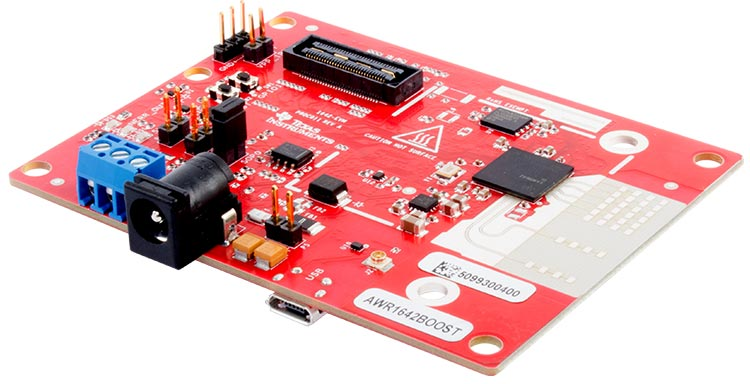
\includegraphics [width=0.5 \textwidth]{imgs/chapter4/awr1642.jpg}}
\caption{Texas Instruments AWR1642BOOST evaluation board}
\label{fig:awr}
\end{figure}

\subsection{}

\section{Turtlebot2}
\section{Software}
The software used in this project is divided in three stages. First one is the interface between the radar board TLV data and the ROS message format. Then a filtering operation to remove false detections. 
\subsection{Interface Between Radar and ROS?}


\section{Summary}   

